% --------------------------------------------------------------------
\documentclass{standalone}

\usepackage{mathtools}

\usepackage{tikz}

\usetikzlibrary{decorations.markings}
\usetikzlibrary{arrows}
\usetikzlibrary{arrows.meta}
\usetikzlibrary{shapes.geometric}

\begin{document}
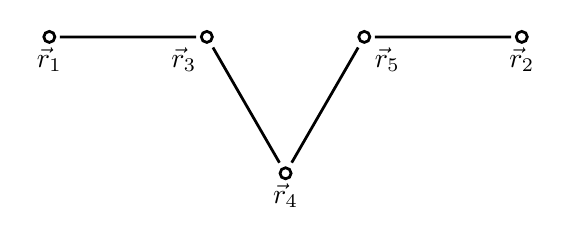
\begin{tikzpicture}[baseline, line width=1pt, scale=1.0]

  \begin{scope}[xshift=0.0cm, yshift=0.0cm]

  \draw (0,0) node [name=r1] {};
  \draw (6,0) node[name=r2] {};
  \draw (2,0) node[name=r3] {};
  \draw (3,-1.7320508075688772) node[name=r4] {};
  \draw (3,0) node[name=rX] {};
  \draw (4,0) node[name=r5] {};

  %\draw [-Stealth] (r1) -- node[midway, above] {$\vec{v}_1$} (r3);
  %\draw [-{Stealth[sep=-4pt]}] (r3) -- node[midway, above] {$\vec{v}_2$} (rX);
  %\draw [-Stealth] (rX) -- node[midway, right] {$\vec{v}_3$} (r4);
  \draw [-] (r1) -- (r3) -- (r4) -- (r5) -- (r2);
  
  \draw (r1) circle [radius=2pt, fill=black!40];
  \draw (r2) circle [radius=2pt, fill=black!40];
  \draw (r3) circle [radius=2pt, fill=black!40];
  \draw (r4) circle [radius=2pt, fill=black!40];
  \draw (r5) circle [radius=2pt, fill=black!40];
  
  \draw (r1) node[below] {$\vec{r}_1$};
  \draw (r2) node[below] {$\vec{r}_2$};
  \draw (r3) node[below left] {$\vec{r}_3$};
  \draw (r4) node[below] {$\vec{r}_4$};
  \draw (r5) node[below right] {$\vec{r}_5$};

  \end{scope}

\end{tikzpicture}
\end{document}
